\chapter{Diseño del sistema: Arquitectura, tecnologías y decisiones clave}\label{cap:disenio}

Este capítulo profundiza en el \textbf{diseño del sistema}, abarcando desde su \textbf{arquitectura general} y la \textbf{elección de tecnologías y frameworks}, hasta el \textbf{diseño de la base de datos} y la \textbf{API}. También se detallan el \textbf{diseño de la interfaz de usuario (UI)} y la \textbf{experiencia de usuario (UX)}, elementos cruciales para garantizar una aplicación intuitiva y accesible.

\section{Decisiones de diseño y arquitectura: Cimientos del sistema}

Esta sección es fundamental, ya que explica la \textbf{arquitectura general del sistema}, definiendo cómo se organizan sus componentes y cómo interactúan. La elección arquitectónica es decisiva para la \textbf{escalabilidad, mantenibilidad y robustez} de la aplicación a largo plazo.

\subsection{El Backend como pilar central}

Desde el inicio del proyecto, el \textbf{diseño del backend} se conceptualizó como la \textbf{piedra angular del sistema}. Dada la complejidad de la lógica de negocio y la gestión de datos, se priorizó una \textbf{infraestructura robusta y escalable} capaz de manejar eficientemente las operaciones principales. Esta decisión asegura la \textbf{estabilidad, rendimiento y seguridad}, independientemente de la interfaz de usuario.

\subsection{Arquitectura de Microservicios: Flexibilidad y escalabilidad}

Para cumplir con los exigentes requisitos de escalabilidad, flexibilidad y mantenibilidad a largo plazo, se optó por una \textbf{arquitectura basada en microservicios} para el backend. Esta elección permite descomponer la aplicación en \textbf{componentes independientes y débilmente acoplados}, cada uno con una funcionalidad de negocio específica.


\begin{table}[H]
    \centering
    \label{tab:monolitico_vs_microservicios_checks}
    \begin{tabular}{|p{4cm}|c|c|}
        \hline
        \textbf{Característica} & \textbf{Arquitectura Monolítica} & \textbf{Arquitectura de Microservicios} \\
        \hline
        \textbf{Velocidad de Desarrollo Inicial} & \checkmark\checkmark\checkmark & \checkmark \\
        \hline
        \textbf{Escalabilidad Independiente} & & \checkmark\checkmark\checkmark \\
        \hline
        \textbf{Mantenibilidad a Largo Plazo} & \checkmark & \checkmark\checkmark\checkmark \\
        \hline
        \textbf{Flexibilidad Tecnológica (Políglota)} & & \checkmark\checkmark\checkmark \\
        \hline
        \textbf{Resiliencia (Aislamiento de Fallos)} & \checkmark & \checkmark\checkmark\checkmark \\
        \hline
        \textbf{Despliegues Rápidos y Frecuentes} & \checkmark & \checkmark\checkmark\checkmark \\
        \hline
        \textbf{Complejidad Operacional} & \checkmark\checkmark\checkmark & \checkmark \\
        \hline
        \textbf{Coste Inicial de Infraestructura} & \checkmark\checkmark\checkmark & \checkmark \\
        \hline
        \textbf{Adaptabilidad a Cambios} & \checkmark & \checkmark\checkmark\checkmark \\
        \hline
        \textbf{Independencia de Equipos} & \checkmark & \checkmark\checkmark\checkmark \\
        \hline
    \end{tabular}
    \caption{Comparativa: Arquitectura Monolítica vs. Microservicios}
\end{table}

Comparada con una arquitectura monolítica, los microservicios ofrecen ventajas significativas. Mientras que un monolito puede ser más sencillo de implementar inicialmente, su mantenimiento y escalabilidad eficiente se complican a medida que la aplicación crece. Los microservicios, en cambio, fomentan una mayor \textbf{modularidad y reutilización}, facilitando el \textbf{desarrollo ágil y la integración continua}. Cada microservicio puede ser \textbf{desarrollado, desplegado y escalado de forma independiente}, lo que agiliza la implementación de nuevas funcionalidades y la adaptación a cambios en los requisitos.

\subsection{Separación Backend-Frontend: Comunicación vía API REST}

Una decisión arquitectónica fundamental, coherente con los microservicios, es la \textbf{completa separación entre el backend y el frontend}. Esto implica que el backend funciona como una entidad autónoma, sin conocimiento directo de la presentación al usuario. Esta independencia ofrece ventajas esenciales:

\begin{itemize}
    \item \textbf{Flexibilidad de Desarrollo:} Permite que equipos de frontend y backend trabajen en paralelo con distintas tecnologías, acelerando el ciclo de desarrollo.
    \item \textbf{Reusabilidad de Servicios:} Un mismo backend puede soportar múltiples interfaces de usuario (web, móvil), evitando la duplicidad de lógica de negocio.
    \item \textbf{Escalabilidad Horizontal Independiente:} Facilita el escalado individual de cada componente (frontend o backend) según la demanda, optimizando los recursos.
    \item \textbf{Mantenibilidad Mejorada:} Cambios en una capa (ej. refactorización del frontend) no afectan directamente a la otra, reduciendo riesgos y simplificando el mantenimiento.
    \item \textbf{Seguridad Robusta:} Permite implementar medidas de seguridad específicas y más robustas para cada componente, especialmente en el backend, que maneja datos sensibles.
\end{itemize}

La comunicación exclusiva entre el backend y el frontend se realiza mediante una \textbf{API REST (Representational State Transfer)}~\ref{fig:rest_architecture}. La elección de REST se basa en su \textbf{simplicidad, naturaleza sin estado y amplia adopción}, lo que facilita la integración e interoperabilidad. La API REST define un conjunto de \textit{endpoints} y utiliza un formato estandarizado, generalmente \textbf{JSON (JavaScript Object Notation)}, para el intercambio de datos.

\begin{figure}[H]
    \centering
    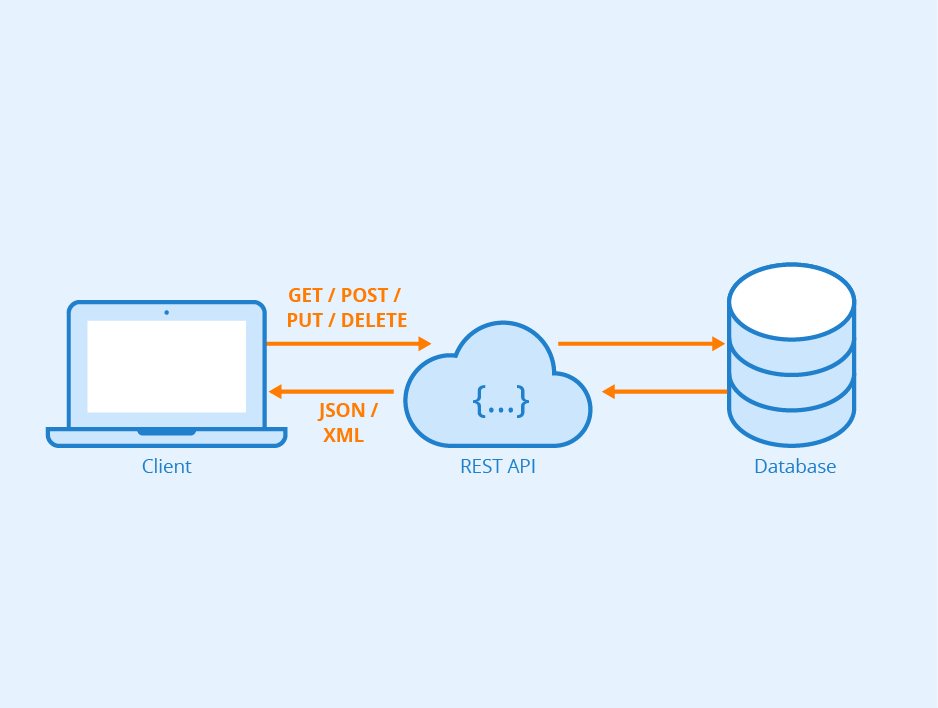
\includegraphics[width=0.8\textwidth, trim=0cm 2cm 0cm 2cm, clip]{figures/06_rest.png}
    \caption{Comunicación Backend-Frontend a través de API REST}
    \label{fig:rest_architecture}
\end{figure}

\section{Backend: Diseño y tecnologías clave}

Una vez definidos los requisitos del sistema, se procedió a diseñar el \textbf{backend} de la aplicación, siguiendo la arquitectura de microservicios, donde cada servicio gestiona una funcionalidad específica.

\subsection{Servicios del Backend identificados}

Los servicios identificados para cumplir con los requisitos del sistema son:
\begin{itemize}
    \item \textbf{Servicio de Autenticación y Autorización (Auth Service):} Gestiona el acceso, registro, inicio de sesión y permisos de usuarios.
    \item \textbf{Servicio de Gestión de Usuarios (User Service):} Responsable de la creación, actualización y eliminación de perfiles de usuario.
    \item \textbf{Servicio de Gestión de Horarios y Calendario (Schedule Consumer Service):} Obtiene y administra el horario académico desde el sistema de la UGR.
    \item \textbf{Servicio de Notificaciones (Mail Service):} Envía notificaciones a los usuarios (creación de eventos, registro completado, reseteo de contraseña, etc.).
    \item \textbf{Servicio de Matriculaciones (Academic Subscription Service):} Gestiona las matriculaciones de usuarios en asignaturas y grupos, actualiza el horario personalizado y crea eventos adicionales.
\end{itemize}

Cada servicio se implementa como una aplicación independiente para una mayor flexibilidad y escalabilidad. La comunicación entre ellos se realiza tanto vía \textbf{API REST} como mediante \textbf{eventos a través de RabbitMQ}, lo que crea una arquitectura más robusta y desacoplada. Un \textbf{API Gateway} actúa como punto de entrada para todas las solicitudes del frontend, enrutándolas, gestionando la autenticación/autorización y aportando una capa adicional de seguridad.

\subsection{Tecnologías y Frameworks del Backend}

Para el desarrollo del backend, se eligió el stack tecnológico de \textbf{Java con Spring Boot}, que ofrece ventajas significativas para microservicios:

\begin{itemize}
    \item \textbf{Spring Boot:} Facilita la creación de aplicaciones Java independientes y productivas con mínima configuración.
    \item \textbf{Spring Security:} Proporciona un marco completo para una autenticación y autorización robustas.
    \item \textbf{Spring Data JPA:} Simplifica el acceso a bases de datos relacionales mediante JPA.
    \item \textbf{Spring Cloud:} Ofrece herramientas para construir aplicaciones distribuidas (descubrimiento de servicios, configuración centralizada, gestión de circuitos).
\end{itemize}

Spring Framework es una tecnología líder en Java, con un vasto ecosistema de herramientas y bibliotecas que facilitan la creación de aplicaciones robustas y escalables. La elección de Java como lenguaje de programación capitaliza un lenguaje maduro, ampliamente adoptado, con una gran comunidad, un ecosistema rico y compatibilidad con diversas plataformas y sistemas operativos, además de su velocidad de ejecución \cite{speed_comparison} en comparación con otros lenguajes usados en backend, reflejado en la figura~\ref{fig:programming_languages_speed}.

\begin{figure}[H]
    \centering
    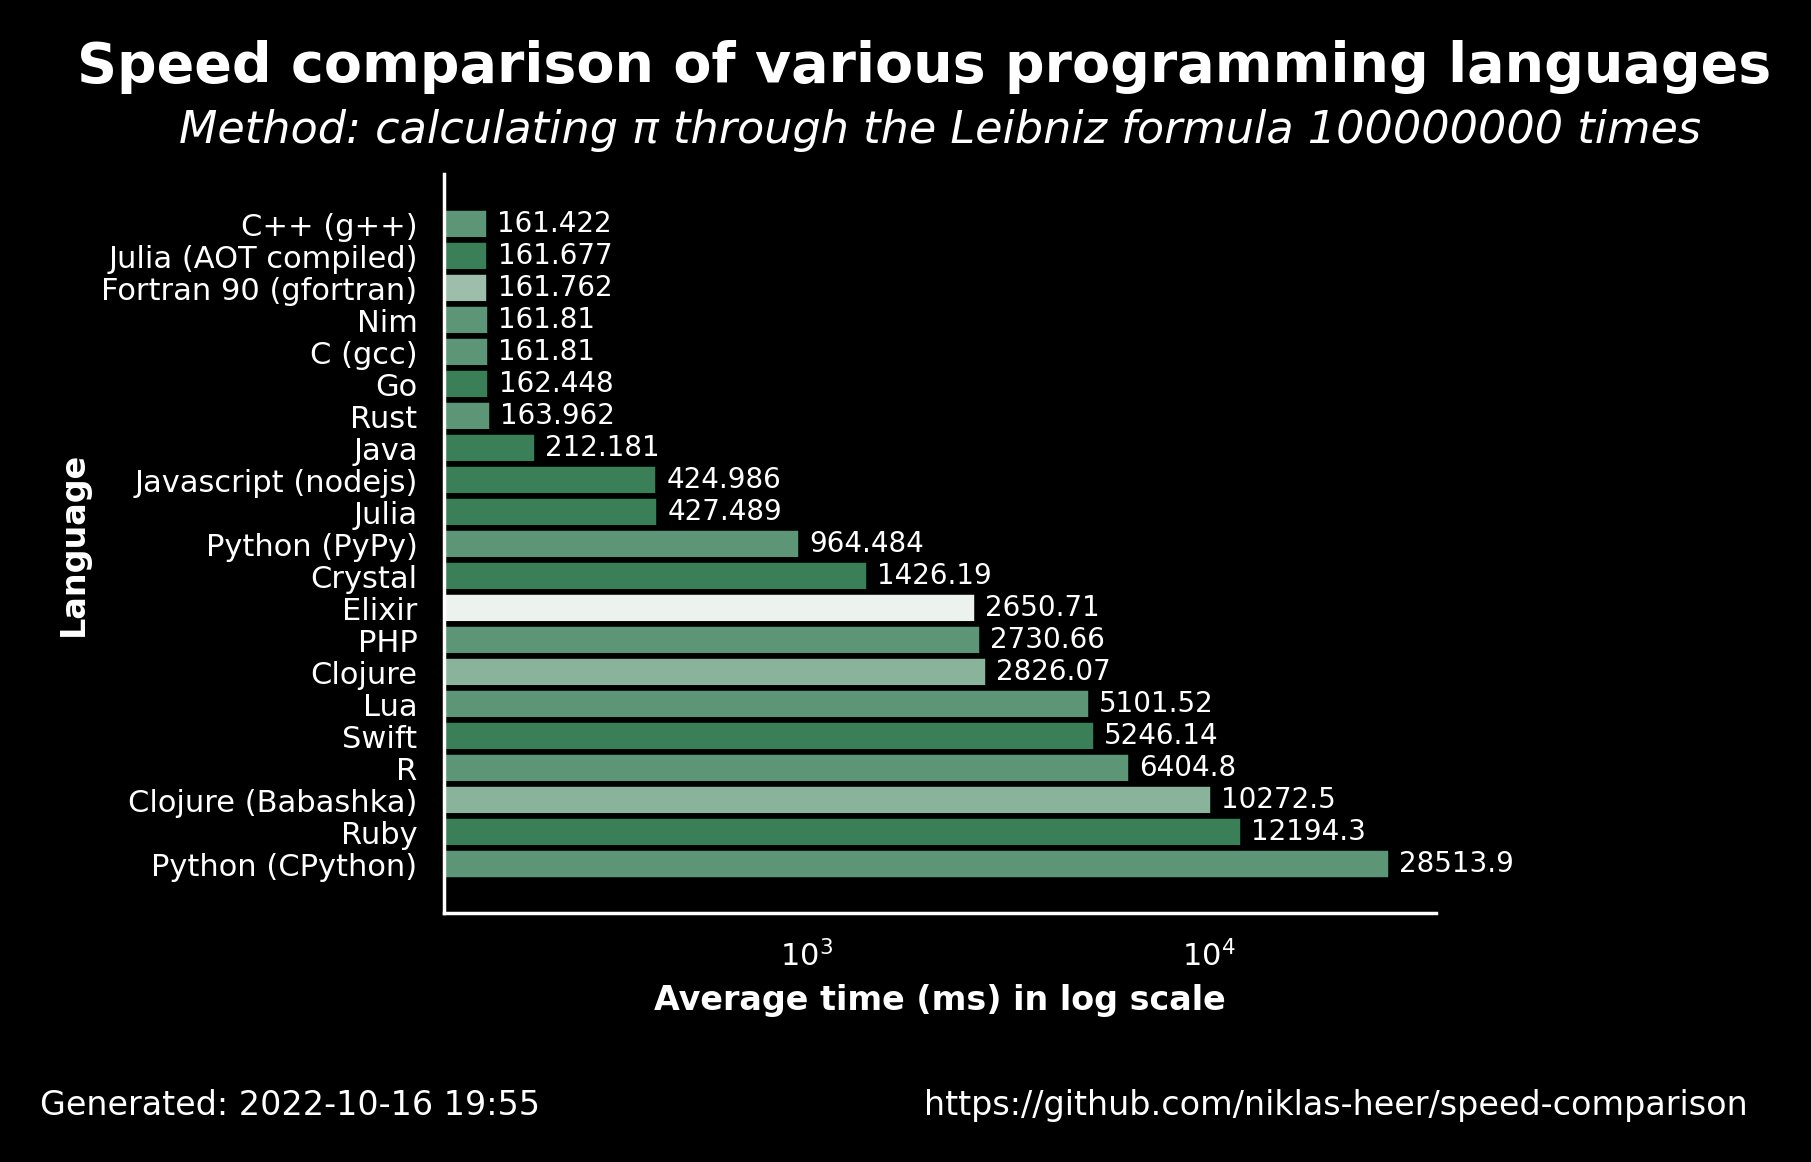
\includegraphics[width=0.9\textwidth]{figures/06_comp.png}
    \caption{Comparativa de velocidades entre lenguajes de programación}
    \label{fig:programming_languages_speed}
\end{figure}

Para el descubrimiento de servicios en esta arquitectura de microservicios, se integró \textbf{Eureka}, que permite a los servicios registrarse y descubrirse entre sí en la red. Sus ventajas incluyen:
\begin{itemize}
    \item \textbf{Descubrimiento de Servicios:} Facilita la comunicación y el enrutamiento de solicitudes entre microservicios.
    \item \textbf{Escalabilidad:} Permite añadir o eliminar instancias de servicios sin reconfiguración manual.
    \item \textbf{Resiliencia:} Ofrece mecanismos para manejar fallos de servicios, manteniendo la aplicación funcional.
    \item \textbf{Configuración Centralizada:} Simplifica la administración y el despliegue al centralizar la configuración de los servicios.
\end{itemize}

Como base de datos relacional para ``User Service'' y ``Schedule Consumer Service'' se optó por \textbf{MySQL}, un sistema de gestión de bases de datos ampliamente utilizado y confiable, que ofrece robustez, escalabilidad y un sólido soporte para transacciones. MySQL es ideal para aplicaciones que requieren integridad referencial y consultas complejas, lo que lo convierte en una excelente opción para manejar los datos de usuarios y horarios académicos.

La comunicación asíncrona y desacoplada entre servicios se logra mediante \textbf{RabbitMQ}, un sistema de mensajería ampliamente utilizado que proporciona alta disponibilidad, escalabilidad y fiabilidad en la entrega de mensajes, siendo una excelente elección para la arquitectura de microservicios. Se eligió RabbitMQ sobre alternativas como Kafka o ActiveMQ por su simplicidad, facilidad de uso, amplia adopción y compatibilidad.

Finalmente, \textbf{Docker} se seleccionó para la \textbf{contenedorización de los servicios}, permitiendo una fácil implementación y escalabilidad. Docker proporciona un entorno aislado y reproducible para cada servicio, simplificando el despliegue en diferentes entornos (desarrollo, pruebas, producción) y mejorando la portabilidad.

Tras la selección de tecnologías y la definición de las interacciones entre los servicios, se establece la siguiente arquitectura general del backend en la figura~\ref{fig:backend_architecture}:

\begin{figure}[H]
    \centering
    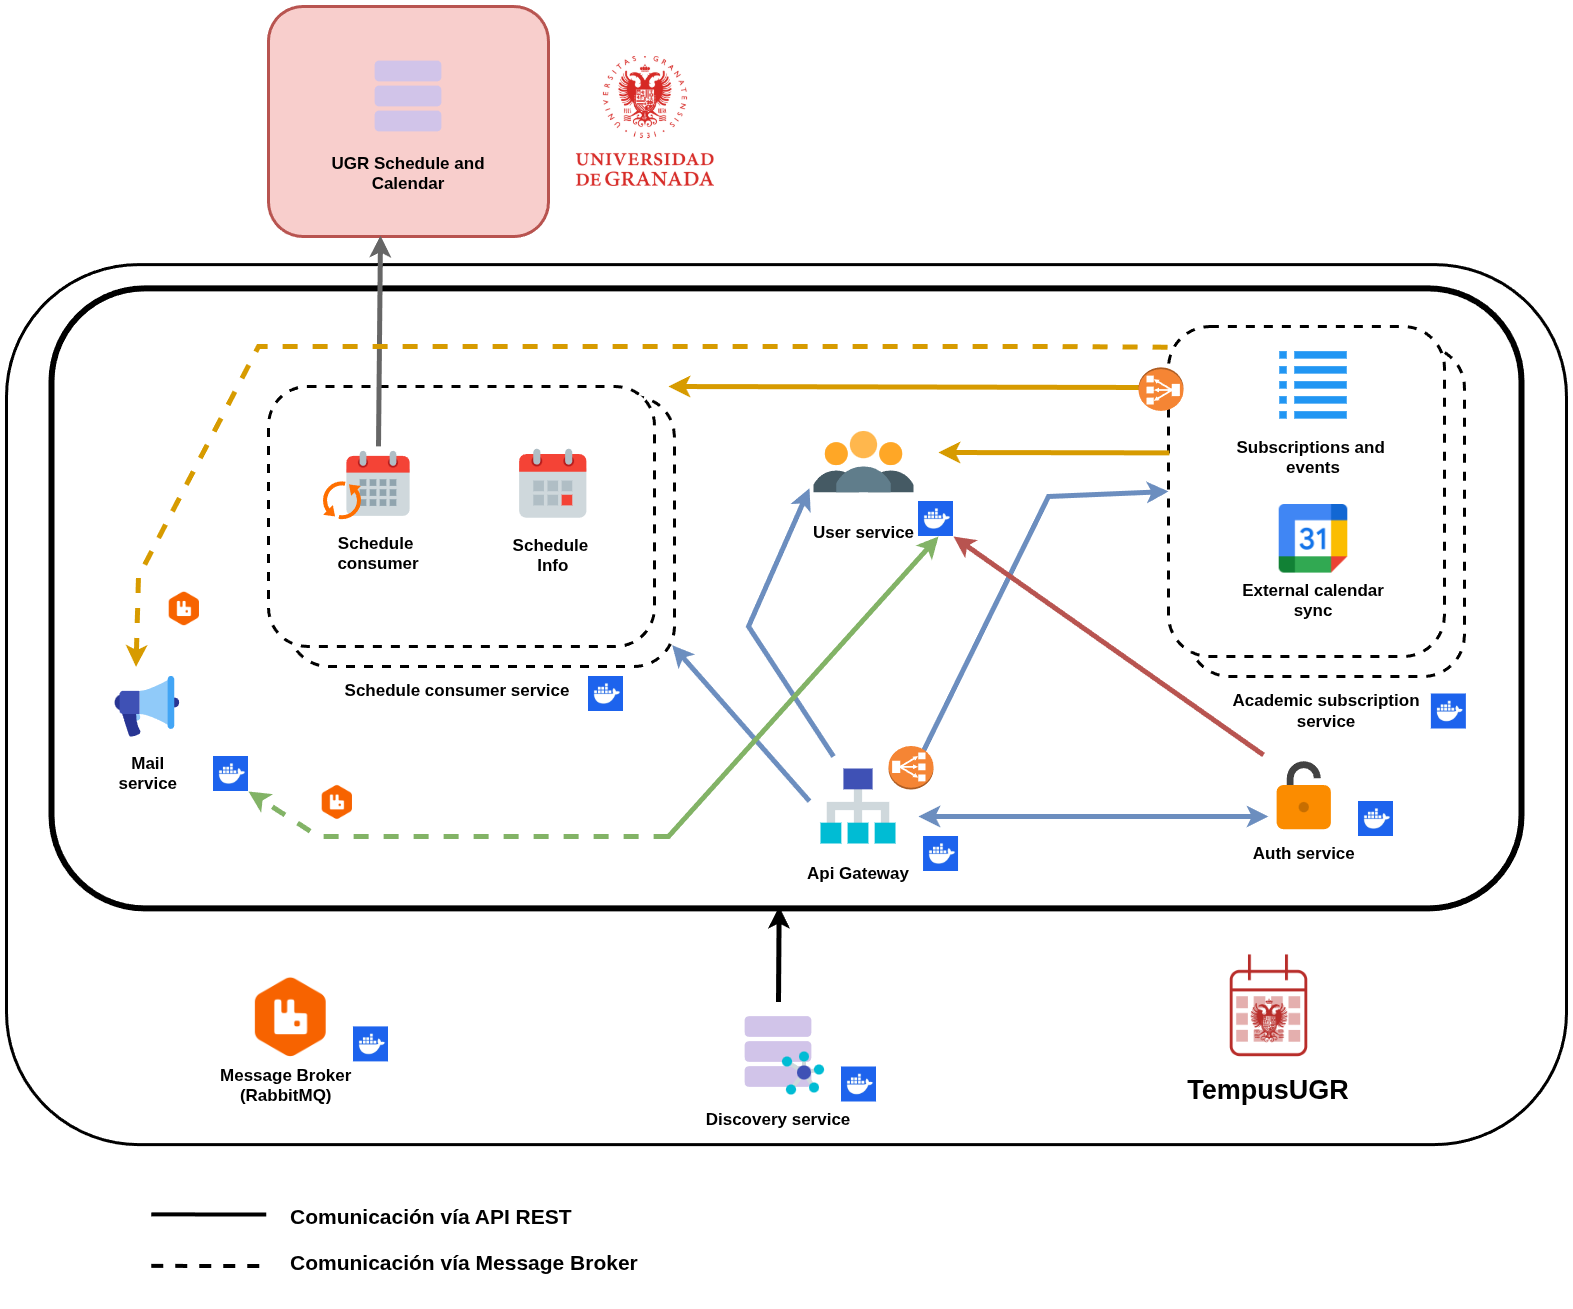
\includegraphics[width=1\textwidth]{figures/06_arq.png}
    \caption{Arquitectura general del Backend}
    \label{fig:backend_architecture}
\end{figure}

\subsubsection{Comunicaciones entre servicios}

Como se observa en el diagrama, las comunicaciones se distinguen por dos tipos principales:

\begin{itemize}
    \item \textbf{Comunicación vía API REST (Líneas Sólidas Negras y de Colores):}
    Este es el método principal para las interacciones síncronas, donde un servicio realiza una solicitud directa a otro y espera una respuesta inmediata. El \textbf{API Gateway} actúa como el punto de entrada para todas las solicitudes externas (provenientes de \texttt{TempusUGR}) y las enruta a los servicios correspondientes.
    \begin{itemize}
        \item \textbf{API Gateway $\leftrightarrow$ Auth Service:} El \textbf{API Gateway} se comunica con el \textbf{Auth Service} para gestionar la autenticación y autorización de los usuarios en cada solicitud entrante, asegurando que solo usuarios válidos y con permisos adecuados accedan a los recursos del sistema.
        \item \textbf{API Gateway $\leftrightarrow$ User Service:} Las solicitudes relacionadas con la gestión de usuarios (ej., creación, consulta, modificación de perfiles) son enrutadas desde el \textbf{API Gateway} al \textbf{User Service}.
        \item \textbf{API Gateway $\leftrightarrow$ Academic Subscription Service:} Las peticiones para gestionar suscripciones académicas, eventos personalizados y la sincronización con sistemas de calendario externos (ej., Google Calendar) se dirigen desde el \textbf{API Gateway} al \textbf{Academic Subscription Service}.
        \item \textbf{API Gateway $\leftrightarrow$ Schedule Consumer Service:} Las solicitudes para obtener información sobre horarios académicos (ej., buscar horarios de titulaciones, asignaturas) son enrutadas desde el \textbf{API Gateway} al \textbf{Schedule Consumer Service}.
        \item \textbf{Academic Subscription Service $\leftrightarrow$ User Service:} El \textbf{Academic Subscription Service} necesita comunicarse con el \textbf{User Service} para obtener información detallada de los usuarios, como sus identificadores o datos de perfil, cuando gestiona las suscripciones o eventos vinculados a ellos.
        \item \textbf{Academic Subscription Service $\leftrightarrow$ Schedule Consumer Service:} El \textbf{Academic Subscription Service} interactúa con el \textbf{Schedule Consumer Service} para obtener la información de las asignaturas matriculadas por los usuarios, como parte del proceso de construcción de sus horarios personalizados o la validación de suscripciones.
    \end{itemize}

    \item \textbf{Comunicación vía Message Broker (RabbitMQ - Líneas Discontinuas):}
    Para la comunicación asíncrona y el desacoplamiento entre servicios, se utiliza un \textbf{Message Broker (RabbitMQ)}. Este patrón es ideal para notificaciones, procesamiento en segundo plano y cuando un servicio necesita informar a otros sin esperar una respuesta inmediata.
    \begin{itemize}
        \item \textbf{Academic Subscription Service $\rightarrow$ Message Broker $\rightarrow$ Mail Service:} Cuando se producen eventos significativos en el \textbf{Academic Subscription Service} (ej., creación de una nueva suscripción, adición de un evento personalizado), este publica un mensaje en el Message Broker. El \textbf{Mail Service} consume estos mensajes para enviar notificaciones por correo electrónico a los usuarios implicados de forma asíncrona.
        \item \textbf{User Service $\rightarrow$ Message Broker $\rightarrow$ Mail Service:} De manera similar, cuando se realizan acciones relacionadas con el perfil de usuario en el \textbf{User Service} (ej., registro de un nuevo usuario, reseteo de contraseña), este publica mensajes en el Message Broker. El \textbf{Mail Service} los consume para enviar comunicaciones relevantes a los usuarios, como correos de bienvenida o confirmaciones.
    \end{itemize}
\end{itemize}

Además de estos mecanismos de comunicación explícitos, es importante destacar el papel del \textbf{Discovery Service (Eureka)}. Aunque no se muestra directamente en el flujo de datos del diagrama, es fundamental para que los microservicios puedan encontrarse y comunicarse entre sí de manera dinámica y resiliente, sin necesidad de direcciones IP o puertos codificados rígidamente.

Esta combinación de comunicación síncrona (API REST a través de API Gateway) y asíncrona (RabbitMQ) permite construir una arquitectura \textbf{robusta, escalable y mantenible}, donde los servicios pueden evolucionar de forma independiente y reaccionar a los eventos del sistema de manera eficiente y desacoplada.

\subsubsection{Obtención de horarios académicos}

El \textbf{Servicio de Horarios y Calendario (Schedule Consumer Service)} es el encargado principal de recolectar la información de horarios académicos. Para ello, se emplea una técnica de \textbf{web scraping} dirigida a la web oficial de grados de la Universidad de Granada (UGR). Este proceso consiste en la extracción automatizada de datos estructurados desde páginas web.

El flujo de obtención de horarios sigue los siguientes pasos:
\begin{enumerate}
    \item \textbf{Identificación de URLs:} El servicio está configurado con las URLs de las páginas web de grados de la UGR que contienen la información de los horarios.
    \item \textbf{Raspado de datos:} Se utiliza un algoritmo de web scraping para navegar por estas páginas, identificar los elementos HTML que contienen la información relevante (ej., tablas de horarios, nombres de asignaturas, grupos, profesores, aulas y fechas) y extraerlos de forma programática.
    \item \textbf{Procesamiento y Normalización:} Los datos extraídos, que inicialmente pueden estar en un formato inconsistente o no estructurado, son procesados y normalizados para ajustarse al modelo de datos definido en la base de datos del \textbf{Schedule Consumer Service} (entidades \texttt{Grade}, \texttt{Subject}, \texttt{Subject\_group}, \texttt{Class\_info}). Este paso es crucial para asegurar la coherencia y la integridad de la información.
    \item \textbf{Almacenamiento:} Una vez normalizados, los datos se persisten en la base de datos \textbf{MySQL} asociada al servicio.
\end{enumerate}

Esta estrategia de web scraping permite mantener la base de datos de horarios académicos actualizada con la información publicada por la UGR, garantizando que el sistema TempusUGR opere con los datos más recientes y precisos para la gestión de horarios y matriculaciones.

\subsubsection{Balanceo de Carga}

Como se refleja en la arquitectura, el sistema se ha preparado para levantar varias instancias de los servicios ``Academic Subscription Service'' y ``Schedule Consumer Service''. Esto permite distribuir la carga de trabajo entre múltiples instancias, mejorando la capacidad de respuesta y la disponibilidad del sistema. El balanceo de carga se gestiona a través del \textbf{API Gateway} y \textbf{Academic Subscription Service}, que enrutan las solicitudes entrantes a la instancia adecuada del servicio, basándose en criterios como la disponibilidad, la carga actual o el tipo de solicitud.
\newline\newline
EL algoritmo de balanceo de carga utilizado es el \textbf{Round Robin}, que distribuye las solicitudes entrantes de manera equitativa entre todas las instancias disponibles. Este enfoque es simple y efectivo, especialmente en escenarios donde las instancias tienen capacidades similares y se espera una carga uniforme.

\subsection{Modelado de la base de datos}

Una vez definidos los requisitos de información del sistema, y los sitemas de gestión de bases de datos a usar en cada servicio, se procedió a diseñar el modelo de datos~\ref{fig:user_service_er} para cada uno de los servicios del backend. A continuación se muestran los diagramas de entidad-relación (ER) para cada uno de estos:

\begin{figure}[H]
    \centering
    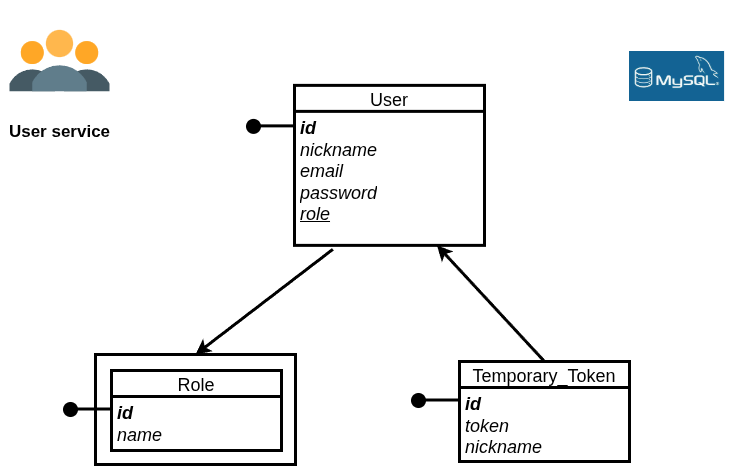
\includegraphics[width=0.7\textwidth]{figures/06_user_db.png}
    \caption{Modelo de datos del Servicio de Usuarios}
    \label{fig:user_service_er}
\end{figure}

A continuación, se detalla la estructura y propósito de cada entidad:

\begin{itemize}
    \item \textbf{Entidad User:}
    Esta entidad representa a los usuarios del sistema y es el núcleo del servicio. Almacena la información esencial para la identificación y autenticación.
    \begin{itemize}
        \item \textbf{id}: Clave primaria única para cada usuario.
        \item \textbf{nickname}: Nombre de usuario único, utilizado para la identificación en el sistema.
        \item \textbf{email}: Dirección de correo electrónico del usuario, también única y utilizada para comunicaciones y recuperación de cuenta.
        \item \textbf{password}: Contraseña del usuario, almacenada de forma segura (normalmente como un hash).
        \item \textbf{role}: Hace referencia al rol del usuario, estableciendo una relación con la entidad \textbf{Role}.
    \end{itemize}

    \item \textbf{Entidad Role:}
    Define los distintos roles o perfiles que un usuario puede tener dentro del sistema, lo que permite implementar un control de acceso basado en roles (RBAC).
    \begin{itemize}
        \item \textbf{id}: Clave primaria única para cada rol.
        \item \textbf{name}: Nombre del rol (\texttt{ROLE\_INACTIVE}, \texttt{ROLE\_STUDENT}, \texttt{ROLE\_TEACHER}, \texttt{ROLE\_ADMIN}).
    \end{itemize}
    La relación entre \textbf{User} y \textbf{Role} es de uno a muchos (un rol puede ser asignado a múltiples usuarios), o de muchos a muchos si un usuario pudiera tener varios roles (aunque el diagrama sugiere una relación de uno a muchos a través del campo \texttt{role} en \textbf{User}). Para mayor claridad en el futuro, se podría especificar el tipo de relación.

    \item \textbf{Entidad Temporary\_Token:}
    Esta entidad se utiliza para gestionar tokens de un solo uso, comúnmente empleados para procesos como la recuperación de contraseña o la verificación de correo electrónico.
    \begin{itemize}
        \item \textbf{id}: Clave primaria única para cada token temporal.
        \item \textbf{token}: El valor único del token generado.
        \item \textbf{nickname}: Hace referencia al \textbf{nickname} del usuario al que está asociado el token, estableciendo una relación directa con la entidad \textbf{User}.
    \end{itemize}
    Esta relación implica que cada token temporal está asociado a un usuario específico.
\end{itemize}

Este diseño de base de datos~\ref{fig:schedule_service_er} proporciona una estructura sólida para el \textbf{Servicio de Gestión de Usuarios}, permitiendo una gestión eficiente y segura de la información de los usuarios, sus permisos y los mecanismos de autenticación adicionales.

\begin{figure}[H]
    \centering
    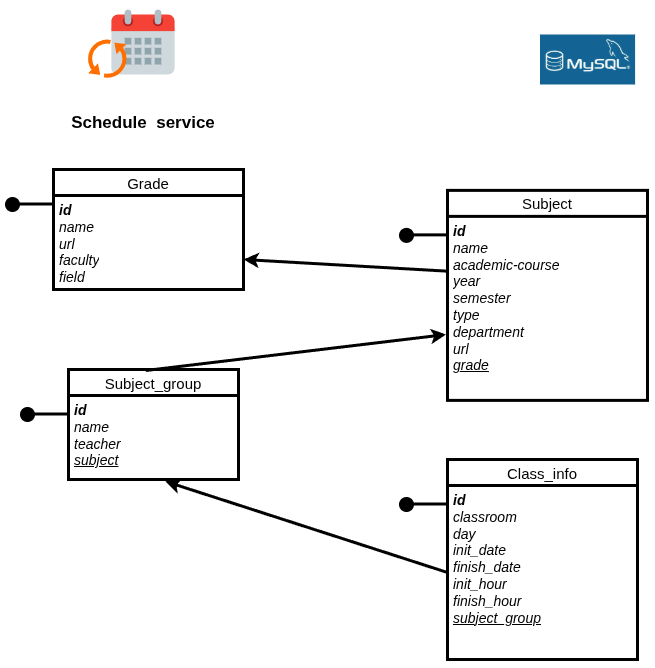
\includegraphics[width=0.7\textwidth]{figures/06_calendar_db.png}
    \caption{Modelo de datos del Servicio de Horarios y Calendario}
    \label{fig:schedule_service_er}
\end{figure}

A continuación, se describen las entidades y sus relaciones:

\begin{itemize}
    \item \textbf{Entidad Grade (Grado):}
    Representa las diferentes titulaciones académicas de las que se obtienen los horarios.
    \begin{itemize}
        \item \textbf{id}: Clave primaria única para cada titulación.
        \item \textbf{name}: Nombre completo de la titulación (ej., "Grado en Ingeniería Informática").
        \item \textbf{url}: URL o identificador del recurso externo de donde se obtienen los datos de la titulación.
        \item \textbf{faculty}: Facultad a la que pertenece la titulación.
        \item \textbf{field}: Área de conocimiento o campo de estudio de la titulación.
    \end{itemize}

    \item \textbf{Entidad Subject (Asignatura):}
    Contiene la información de las asignaturas que forman parte de las titulaciones.
    \begin{itemize}
        \item \textbf{id}: Clave primaria única para cada asignatura.
        \item \textbf{name}: Nombre de la asignatura.
        \item \textbf{academic-course}: Curso académico al que pertenece la asignatura.
        \item \textbf{year}: Año del plan de estudios en el que se imparte la asignatura.
        \item \textbf{semester}: Semestre en el que se imparte la asignatura.
        \item \textbf{type}: Tipo de asignatura (ej., ``Obligatoria'', ``Optativa'').
        \item \textbf{department}: Departamento responsable de la asignatura.
        \item \textbf{url}: URL o identificador del recurso externo de donde se obtienen los datos de la asignatura.
        \item \textbf{grade}: Clave foránea que referencia a la entidad \textbf{Grade}, indicando a qué titulación pertenece la asignatura (relación uno a muchos: una titulación tiene muchas asignaturas).
    \end{itemize}

    \item \textbf{Entidad Subject\_group (Grupo de Asignatura):}
    Representa los diferentes grupos en los que se divide una asignatura para su impartición.
    \begin{itemize}
        \item \textbf{id}: Clave primaria única para cada grupo de asignatura.
        \item \textbf{name}: Nombre o identificador del grupo (ej., "Grupo 1", "Grupo A").
        \item \textbf{teacher}: Profesor o profesores asignados a este grupo.
        \item \textbf{subject}: Clave foránea que referencia a la entidad \textbf{Subject}, indicando a qué asignatura pertenece este grupo (relación uno a muchos: una asignatura tiene muchos grupos).
    \end{itemize}

    \item \textbf{Entidad Class\_info (Información de Clase):}
    Almacena los detalles específicos de cada sesión de clase para un grupo de asignatura.
    \begin{itemize}
        \item \textbf{id}: Clave primaria única para cada entrada de clase.
        \item \textbf{classroom}: Aula o lugar donde se imparte la clase.
        \item \textbf{day}: Día de la semana en que se imparte la clase.
        \item \textbf{init\_date}: Fecha de inicio de la clase o del período de clases.
        \item \textbf{finish\_date}: Fecha de finalización de la clase o del período de clases.
        \item \textbf{init\_hour}: Hora de inicio de la clase.
        \item \textbf{finish\_hour}: Hora de finalización de la clase.
        \item \textbf{subject\_group}: Clave foránea que referencia a la entidad \textbf{Subject\_group}, indicando a qué grupo de asignatura pertenece esta clase (relación uno a muchos: un grupo puede tener muchas clases).
    \end{itemize}
\end{itemize}

Este esquema de base de datos~\ref{fig:academic_subscription_service_er} permite al \textbf{Servicio de Horarios y Calendario} organizar y gestionar de manera eficiente toda la información académica necesaria para la composición de los horarios de los usuarios.

\begin{figure}[H]
    \centering
    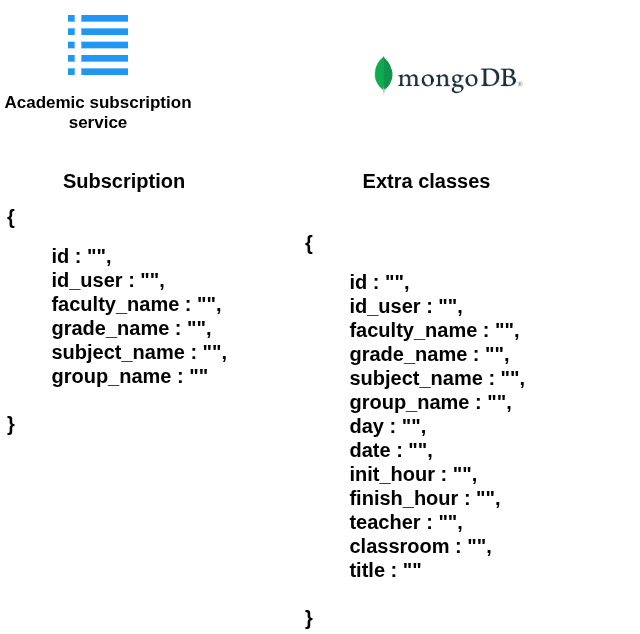
\includegraphics[width=0.7\textwidth, trim=0cm 0cm 2.5cm 0cm, clip]{figures/06_sub_db.png}
    \caption{Modelo de datos del Servicio de Matriculaciones}
    \label{fig:academic_subscription_service_er}
\end{figure}

A continuación, se detalla la estructura esperada de los documentos en cada colección:

\begin{itemize}
    \item \textbf{Colección Subscription:}
    Esta colección almacena las matriculaciones de los usuarios en asignaturas y grupos específicos, reflejando su horario oficial.
    \begin{itemize}
        \item \textbf{id}: Identificador único del documento de suscripción.
        \item \textbf{id\_user}: Identificador del usuario al que pertenece esta suscripción. Permite vincular la suscripción a un usuario específico.
        \item \textbf{faculty\_name}: Nombre de la facultad de la titulación asociada.
        \item \textbf{grade\_name}: Nombre de la titulación a la que se suscribe el usuario.
        \item \textbf{subject\_name}: Nombre de la asignatura a la que el usuario está matriculado.
        \item \textbf{group\_name}: Nombre del grupo de la asignatura al que el usuario está matriculado.
    \end{itemize}
    Esta estructura flexible permite registrar la información de la matriculación sin la rigidez de un esquema relacional fijo, adaptándose a posibles variaciones en los detalles académicos.

    \item \textbf{Colección Extra classes:}
    Esta colección está diseñada para almacenar clases o eventos adicionales que los usuarios puedan crear para su horario personalizado, no directamente vinculados al horario oficial.
    \begin{itemize}
        \item \textbf{id}: Identificador único del documento de clase extra.
        \item \textbf{id\_user}: Identificador del usuario que creó esta clase adicional.
        \item \textbf{faculty\_name}: Nombre de la facultad relacionada con la clase (opcional, para contexto).
        \item \textbf{grade\_name}: Nombre de la titulación relacionada (opcional, para contexto).
        \item \textbf{subject\_name}: Nombre de la asignatura (si aplica, para contexto).
        \item \textbf{group\_name}: Nombre del grupo (si aplica, para contexto).
        \item \textbf{day}: Día de la semana en que se imparte la clase extra.
        \item \textbf{date}: Fecha específica de la clase extra.
        \item \textbf{init\_hour}: Hora de inicio de la clase extra.
        \item \textbf{finish\_hour}: Hora de finalización de la clase extra.
        \item \textbf{teacher}: Nombre del profesor o ponente de la clase extra.
        \item \textbf{classroom}: Aula o lugar donde se imparte la clase extra.
        \item \textbf{title}: Título o descripción breve de la clase extra.
    \end{itemize}
    La flexibilidad de MongoDB es particularmente útil aquí, ya que los campos pueden variar entre documentos de "Extra classes" dependiendo de la naturaleza del evento.
\end{itemize}

La elección de MongoDB para estas colecciones permite una \textbf{rápida inserción y consulta de datos}, así como una \textbf{fácil adaptación a cambios en el esquema de datos} sin requerir migraciones complejas, lo que es ventajoso para la gestión dinámica de las suscripciones y eventos personalizados de los usuarios.

\subsection{Diseño de la API}

El diseño de la API del backend se basa en el principio de \textbf{REST (Representational State Transfer)}, que define un conjunto de convenciones para la creación de servicios web escalables y mantenibles. La API está estructurada en torno a recursos, cada uno representado por una URL única, y utiliza los métodos HTTP estándar para interactuar con estos recursos.
\newline\newline
Para su estandarización se ha seguido la especificación de la \textbf{RFC 7231}\cite{rfc7231}, que define el HyperText Transfer Protocol (HTTP/1.1) y sus métodos, así como las convenciones para la creación de APIs RESTful. Esta especificación proporciona un marco claro para el diseño de APIs, asegurando que sean intuitivas, predecibles y fáciles de consumir por los clientes.
\newline
Además de esta se ha revisado la \textbf{RFC 1738}\cite{rfc1738}, que define el formato de las URLs, asegurando que todas las rutas de la API sigan una estructura coherente y fácil de entender. Esto es crucial para la usabilidad de la API, ya que permite a los desarrolladores comprender rápidamente cómo interactuar con los diferentes recursos del sistema.
\newline\newline
Para hacer pruebas y documentar la API de manera efectiva, se ha utilizado \textbf{Postman}, una herramienta ampliamente adoptada en la comunidad de desarrollo para probar y documentar APIs. Postman permite a los desarrolladores enviar solicitudes HTTP a la API, inspeccionar las respuestas y crear colecciones de pruebas que pueden ser compartidas y reutilizadas. Además, facilita la generación de documentación interactiva de la API, lo que mejora la experiencia del desarrollador al integrar o consumir los servicios.

\subsubsection{Estructura de la API}

En primer lugar, y gracias al uso de un \textbf{API Gateway}, se ha definido una estructura de URL base para la API, que es la siguiente:
\begin{lstlisting}[language=Java]
http://<host>:<port>/calendarugr/v1
\end{lstlisting}
Donde ``\<host\>'' la ip del host donde se despliega la aplicación y ``\<port\>'' es el puerto en el que escucha el API Gateway. Esta estructura base permite una fácil identificación de la versión de la API y proporciona un punto de entrada común para todas las solicitudes. Además en secciones posteriores al implementar https, y al adquirir un dominio de la UGR, esta URL base se actualizará para reflejar el dominio oficial del servicio.
\begin{lstlisting}[language=Java]
https://tempus.ugr.es/calendarugr/v1
\end{lstlisting}

A partir de esta URL base, los diferentes microservicios exponen sus funcionalidades a través de rutas específicas. La API se ha estructurado lógicamente según los servicios del backend, facilitando la comprensión y el uso por parte de los clientes. A continuación, se detallan los principales grupos de endpoints.

\noindent\textbf{Nota sobre Autorización:} Todos los endpoints de la API requieren autenticación y autorización mediante JWT, con las siguientes excepciones que son de acceso público o gestionan la autenticación inicial:
\begin{itemize}
    \item \texttt{/auth/login}
    \item \texttt{/auth/refresh}
    \item \texttt{/user/register}
    \item \texttt{/user/activate}
    \item \texttt{/academic-subscription/ics} (para la descarga pública de calendarios ICS)
    \item \texttt{/academic-subscription/sync-url} (para la obtención de URLs públicas de sincronización)
    \item \texttt{/user/reset-pass-mail}
    \item \texttt{/user/reset-password} 
\end{itemize}

\paragraph{\textbf{Endpoints del Servicio de Usuarios (User Service):}}
Gestionan la administración de usuarios, roles y la recuperación de contraseñas.
\begin{itemize}
    \item \textbf{Administración de Usuarios (Admin Endpoints):}
    \begin{itemize}
        \item \textbf{POST /user/admin/register}
        \newline Descripción: Crea un usuario sin la necesidad de pasar por confirmación de cuenta (para Administrador).
        \newline Cuerpo (JSON):
\begin{lstlisting}[language=bash]
{
  "nickname": "string",
  "email": "string",
  "password": "string",
  "role": {
    "name": "string"
  },
  "notification": true
}
\end{lstlisting}

        \item \textbf{PUT /user/admin/update/\{id\}}
        \newline Descripción: Actualiza la información de un usuario por su ID (para Administrador).
        \newline Cuerpo (JSON):
\begin{lstlisting}[language=bash]
{
  "nickname": "string",
  "email": "string",
  "password": "string",
  "role": {
    "name": "string"
  },
  "notification": true
}
\end{lstlisting}

        \item \textbf{DELETE /user/admin/delete/\{id\}}
        \newline Descripción: Elimina un usuario por su ID.
    \end{itemize}
    
    \item \textbf{Gestión de Roles (Role related):}
    \begin{itemize}
        \item \textbf{POST /user/role/create}
        \newline Descripción: Crea un nuevo rol.
        \newline Cuerpo (JSON):
\begin{lstlisting}[language=bash]
{
  "name": "string"
}
\end{lstlisting}

        \item \textbf{GET /user/role/all}
        \newline Descripción: Obtiene todos los roles disponibles.

        \item \textbf{DELETE /user/role/delete}
        \newline Descripción: Borra un rol existente.
        \newline Cuerpo (JSON):
\begin{lstlisting}[language=bash]
{
  "name": "string"
}
\end{lstlisting}
    \end{itemize}
    
    \item \textbf{Recuperación de Contraseña (Password recovery):}
    \begin{itemize}
        \item \textbf{POST /user/reset-pass-mail}
        \newline Descripción: Solicita el envío de un correo electrónico para el reseteo de contraseña.
        \newline Parámetros de consulta: mail (string)
    \end{itemize}

    \item \textbf{Consulta y Gestión General de Usuarios:}
    \begin{itemize}
        \item \textbf{GET /user/all}
        \newline Descripción: Obtiene la lista completa de usuarios.

        \item \textbf{GET /user/nickname/\{nickname\}}
        \newline Descripción: Obtiene un usuario por su nickname.

        \item \textbf{GET /user/email/\{email\}}
        \newline Descripción: Obtiene un usuario por su dirección de correo electrónico.

        \item \textbf{GET /user/user-info}
        \newline Descripción: Obtiene la información del usuario asociado al token actual.

        \item \textbf{POST /user/register}
        \newline Descripción: Registra un nuevo usuario en el sistema.
        \newline Cuerpo (JSON):
\begin{lstlisting}[language=bash]
{
  "nickname": "string",
  "email": "string",
  "password": "string"
}
\end{lstlisting}

        \item \textbf{POST /user/activate}
        \newline Descripción: Activa una cuenta de usuario utilizando un token de activación.
        \newline Parámetros de consulta: token (string)

        \item \textbf{PUT /user/deactivate}
        \newline Descripción: Desactiva la cuenta del usuario actual.
        \newline Cuerpo (JSON):
\begin{lstlisting}[language=bash]
{
  "currentPassword": "string"
}
\end{lstlisting}

        \item \textbf{PUT /user/nickname}
        \newline Descripción: Actualiza el nickname del usuario actual.
        \newline Cuerpo (JSON):
\begin{lstlisting}[language=bash]
{
  "nickname": "string"
}
\end{lstlisting}

        \item \textbf{PUT /user/role}
        \newline Descripción: Cambia el rol de un usuario.

        \item \textbf{PUT /user/password}
        \newline Descripción: Actualiza la contraseña del usuario actual.
        \newline Cuerpo (JSON):
\begin{lstlisting}[language=bash]
{
  "currentPassword": "string",
  "newPassword": "string"
}
\end{lstlisting}

        \item \textbf{PUT /user/activate-notifications}
        \newline Descripción: Activa las notificaciones para el usuario actual.

        \item \textbf{PUT /user/deactivate-notifications}
        \newline Descripción: Desactiva las notificaciones para el usuario actual.

        \item \textbf{POST /user/email-list}
        \newline Descripción: Obtiene una lista de correos electrónicos de usuarios basándose en una lista de IDs.
        \newline Cuerpo (JSON):
\begin{lstlisting}[language=bash]
[
  "id1",
  "id2"
]
\end{lstlisting}
    \end{itemize}

    \item \textbf{Endpoints del Servicio de Autenticación (Auth Service):}
    Gestionan el proceso de inicio de sesión y la renovación de tokens.
    \begin{itemize}
        \item \textbf{POST /auth/login}
        \newline Descripción: Permite a un usuario iniciar sesión en el sistema.
        \newline Cuerpo (JSON):
\begin{lstlisting}[language=bash]
{
  "email": "string",
  "password": "string"
}
\end{lstlisting}

        \item \textbf{POST /auth/refresh}
        \newline Descripción: Permite renovar un token de acceso utilizando un refresh token.
        \newline Cuerpo (JSON):
\begin{lstlisting}[language=bash]
{
  "refreshToken": "string"
}
\end{lstlisting}
    \end{itemize}

    \item \textbf{Endpoints del Servicio de Correo (Mail Service):}
    Se utilizan para enviar correos electrónicos.
    \begin{itemize}
        \item \textbf{POST /email/send}
        \newline Descripción: Envía un correo electrónico.
        \newline Cuerpo (JSON):
\begin{lstlisting}[language=bash]
{
  "receiver": "string",
  "subject": "string",
  "message": "string"
}
\end{lstlisting}
    \end{itemize}

    \item \textbf{Endpoints del Servicio de Horarios (Schedule Consumer Service):}
    Proporcionan acceso a la información de horarios académicos obtenida mediante web scraping.
    \begin{itemize}
        \item \textbf{GET /schedule-consumer/classes-from-group}
        \newline Descripción: Obtiene las clases de un grupo específico de una asignatura y titulación.
        \newline Parámetros de consulta: grade (string), subject (string), group (string)

        \item \textbf{GET /schedule-consumer/grades}
        \newline Descripción: Obtiene la lista de todas las titulaciones disponibles.

        \item \textbf{GET /schedule-consumer/subjects-groups}
        \newline Descripción: Obtiene las asignaturas y grupos asociados a una titulación específica.
        \newline Parámetros de consulta: grade (string)

        \item \textbf{GET /schedule-consumer/teacher-classes}
        \newline Descripción: Obtiene las clases impartidas por un profesor, buscando por nombre parcial.
        \newline Parámetros de consulta: partialTeacherName (string)
    \end{itemize}

    \item \textbf{Endpoints del Servicio de Matriculaciones Académicas (Academic Subscription Service):}
    Permiten a los usuarios gestionar sus suscripciones a asignaturas y grupos, así como crear y gestionar eventos personalizados.
    \begin{itemize}
        \item \textbf{GET /academic-subscription/classes}
        \newline Descripción: Obtiene las clases a las que el usuario está suscrito.

        \item \textbf{GET /academic-subscription/entire-calendar}
        \newline Descripción: Obtiene el calendario completo del usuario (suscripciones y eventos extra).

        \item \textbf{GET /academic-subscription/subscriptions}
        \newline Descripción: Obtiene las suscripciones activas del usuario.

        \item \textbf{POST /academic-subscription/subscription}
        \newline Descripción: Suscribe al usuario a una asignatura y grupo específicos.
        \newline Cuerpo (JSON):
\begin{lstlisting}[language=bash]
{
  "faculty": "string",
  "grade": "string",
  "subject": "string",
  "group": "string"
}
\end{lstlisting}

        \item \textbf{POST /academic-subscription/subscription-batching}
        \newline Descripción: Permite suscribirse a múltiples asignaturas y grupos en una sola solicitud.
        \newline Cuerpo (JSON):
\begin{lstlisting}[language=bash]
[
  {
    "faculty": "string",
    "grade": "string",
    "subject": "string",
    "group": "string"
  }
]
\end{lstlisting}

        \item \textbf{GET /academic-subscription/ics}
        \newline Descripción: Permite descargar el calendario del usuario en formato ICS.

        \item \textbf{GET /academic-subscription/sync-url}
        \newline Descripción: Obtiene una URL pública para sincronizar el calendario ICS del usuario con otras aplicaciones.

        \item \textbf{DELETE /academic-subscription/subscription-grade}
        \newline Descripción: Borra todas las suscripciones de un usuario para una titulación específica.

        \item \textbf{DELETE /academic-subscription/subscription}
        \newline Descripción: Borra una suscripción específica de un usuario.

        \item \textbf{GET /academic-subscription/group-event}
        \newline Descripción: Obtiene los eventos de grupo (clases extra) creados por el usuario.

        \item \textbf{POST /academic-subscription/group-event}
        \newline Descripción: Inserta una nueva clase extra o evento de grupo para el usuario.
        \newline Cuerpo (JSON):
\begin{lstlisting}[language=bash]
{
  "classroom": "string",
  "day": "string",
  "date": "YYYY-MM-DD",
  "initHour": "HH:MM:SS",
  "finishHour": "HH:MM:SS",
  "groupName": "string",
  "subjectName": "string",
  "teacher": "string",
  "gradeName": "string",
  "facultyName": "string",
  "title": "string"
}
\end{lstlisting}

        \item \textbf{DELETE /academic-subscription/group-event}
        \newline Descripción: Borra un evento de grupo específico por su ID.

        \item \textbf{GET /academic-subscription/faculty-group-event}
        \newline Descripción: Recoge todos los eventos creados por la facultad del usuario.

        \item \textbf{POST /academic-subscription/faculty-event}
        \newline Descripción: Crea un evento a nivel de facultad.
        \newline Cuerpo (JSON):
\begin{lstlisting}[language=bash]
{
  "day": "string",
  "date": "YYYY-MM-DD",
  "initHour": "HH:MM:SS",
  "finishHour": "HH:MM:SS",
  "facultyName": "string",
  "title": "string"
}
\end{lstlisting}

        \item \textbf{DELETE /academic-subscription/faculty-event}
        \newline Descripción: Borra un evento de facultad por su ID.
    \end{itemize}
\end{itemize}

\section{Frontend: Diseño y tecnologías clave} 

El frontend de TempusUGR se ha desarrollado utilizando \textbf{Angular}, un framework de desarrollo web que permite crear aplicaciones de una sola página (SPA) de manera eficiente y escalable. Angular es conocido por su arquitectura basada en componentes, lo que facilita la reutilización de código y la separación de preocupaciones, permitiendo un desarrollo más organizado y mantenible.
\newline\newline
Se alinea con las mejores prácticas de desarrollo web moderno, incluyendo el uso de \textbf{TypeScript} como lenguaje principal, lo que proporciona tipado estático y características avanzadas de programación orientada a objetos. Esto mejora la calidad del código y facilita la detección temprana de errores durante el desarrollo.
\newline\newline
Además, Angular cuenta con un robusto sistema de inyección de dependencias, lo que permite una gestión eficiente de los servicios y componentes, mejorando la modularidad y la testabilidad de la aplicación. También incluye herramientas integradas para el manejo del enrutamiento, la gestión del estado y la comunicación con APIs RESTful, lo que simplifica el desarrollo de aplicaciones complejas.

\subsection{Diseño de la Interfaz y Experiencia del Usuario (UI/UX)}

En cuanto a la parte visual del proyecto, se tuvo en mente desde el principio tener una interfaz usable, intuitiva y accesible, de manera que se facilitara lo máximo posible el acceso a la información del horario personalizado.
\newline\newline
Para ello, se optó por un diseño minimalista~\ref{fig:logo}, con una paleta de colores clara y un uso moderado de imágenes. Además se utilizó la tipografía ``Segoe UI'' por su diseño moderno con letras redondeadas y diseño limpio que se ve bien en pantallas y papel.
\newline
\begin{center}
\begin{minipage}{0.5\textwidth}
    \begin{itemize}
        \item Color primario: \#b82d2a \colorbox[HTML]{b82d2a}{\hspace{1.5em}} \vspace{0.7em}
        \item Color secundario: \#e4afae \colorbox[HTML]{e4afae}{\hspace{1.5em}} \vspace{0.7em}
        \item Color de fondo: \#f5f5f5 \colorbox[HTML]{f5f5f5}{\hspace{1.5em}} \vspace{0.7em}
        \item Color de texto: \#333333 \colorbox[HTML]{333333}{\hspace{1.5em}}
    \end{itemize}
\end{minipage}
\hfill
\begin{minipage}{0.25\textwidth}
    \centering
    \captionsetup{justification=centering}
    
\includegraphics[width=0.8\textwidth]{figures/logo.png}
    \captionof{figure}{Logo de TempusUGR}
    \label{fig:logo}
\end{minipage}
\end{center}

\newpage
El diseño de la interfaz se ha centrado en la usabilidad, asegurando que los usuarios puedan navegar fácilmente por las diferentes secciones de la aplicación. Se han implementado menús claros y botones intuitivos para facilitar la interacción con el sistema. Además, se ha prestado especial atención a la accesibilidad, siguiendo las pautas WCAG (Web Content Accessibility Guidelines) para garantizar que la aplicación sea usable por personas con discapacidades.
\newline\newline
Además se han seguido los diez principios de diseño de Jakob Nielsen\cite{nielsen10principles}, que son:
\begin{enumerate}
    \item \textbf{Visibilidad del estado del sistema:} La aplicación proporciona retroalimentación clara sobre las acciones del usuario, como confirmaciones de suscripciones o errores en la entrada de datos.
    \item \textbf{Coincidencia entre el sistema y el mundo real:} Se utilizan términos y conceptos familiares para los usuarios, evitando jerga técnica innecesaria.
    \item \textbf{Control y libertad del usuario:} Los usuarios pueden deshacer acciones fácilmente, como cancelar una suscripción o eliminar un evento.
    \item \textbf{Consistencia y estándares:} Se mantiene una terminología y diseño coherentes en toda la aplicación.
    \item \textbf{Prevención de errores:} Se implementan validaciones para evitar entradas incorrectas, como fechas inválidas o grupos inexistentes.
    \item \textbf{Reconocimiento en lugar de recuerdo:} Los menús y opciones son visibles y accesibles, reduciendo la carga cognitiva del usuario.
    \item \textbf{Flexibilidad y eficiencia de uso:} La aplicación permite a los usuarios realizar tareas comunes rápidamente mediante atajos y opciones avanzadas.
    \item \textbf{Diseño estético y minimalista:} La interfaz es limpia y sin distracciones innecesarias, enfocándose en la funcionalidad principal.
    \item \textbf{Ayuda a los usuarios a reconocer, diagnosticar y recuperarse de errores:} Se proporcionan mensajes de error claros y sugerencias para resolver problemas comunes.
    \item \textbf{Ayuda y documentación:} Se incluye una sección de ayuda accesible que explica cómo utilizar las principales funcionalidades de la aplicación.
\end{enumerate}